% simple.tex

\documentclass{article}[12pt,a4paper]

\usepackage{hyperref}
\hypersetup{
    colorlinks,
    citecolor=black,
    filecolor=black,
    linkcolor=black,
    urlcolor=black
}

\usepackage{tikz}
\usetikzlibrary{shapes.geometric, arrows}

\tikzstyle{startstop} = [rectangle, rounded corners, minimum width=3cm, minimum height=1cm,text centered, draw=black, fill=red!30]
\tikzstyle{io} = [trapezium, trapezium left angle=70, trapezium right angle=110, minimum width=3cm, minimum height=1cm, text centered, draw=black, fill=blue!30]
\tikzstyle{process} = [rectangle, minimum width=3cm, minimum height=1cm, text centered, text width=3cm, draw=black, fill=orange!30]
\tikzstyle{decision} = [diamond, minimum width=3cm, minimum height=1cm, text centered, draw=black, fill=green!30]
\tikzstyle{arrow} = [thick,->,>=stealth]

\usepackage{listings}
\usepackage{color}
\usepackage{graphicx}
\graphicspath{ {images/} }

\definecolor{codegreen}{rgb}{0,0.6,0}
\definecolor{codegray}{rgb}{0.5,0.5,0.5}
\definecolor{codepurple}{rgb}{0.58,0,0.82}
\definecolor{backcolour}{rgb}{0.95,0.95,0.92}
\definecolor{uigreen}{RGB}{82,170,94}
\definecolor{uiyellow}{RGB}{240,173,78}
\definecolor{uiblue}{RGB}{91,192,222}

\definecolor{lightgray}{rgb}{.9,.9,.9}
\definecolor{darkgray}{rgb}{.4,.4,.4}
\definecolor{purple}{rgb}{0.65, 0.12, 0.82}

\lstdefinelanguage{JavaScript}{
  keywords={typeof, new, true, false, catch, function, return, null, catch, switch, var, if, in, while, do, else, case, break},
  keywordstyle=\color{blue}\bfseries,
  ndkeywords={class, export, boolean, throw, implements, import, this},
  ndkeywordstyle=\color{darkgray}\bfseries,
  identifierstyle=\color{black},
  sensitive=false,
  comment=[l]{//},
  morecomment=[s]{/*}{*/},
  commentstyle=\color{purple}\ttfamily,
  stringstyle=\color{red}\ttfamily,
  morestring=[b]',
  morestring=[b]"
}

\lstset{
   language=JavaScript,
   backgroundcolor=\color{lightgray},
   extendedchars=true,
   basicstyle=\footnotesize\ttfamily,
   showstringspaces=false,
   showspaces=false,
   numbers=left,
   numberstyle=\footnotesize,
   numbersep=9pt,
   tabsize=2,
   breaklines=true,
   showtabs=false,
   captionpos=b
}

\lstdefinestyle{python}{
    backgroundcolor=\color{backcolour},   
    commentstyle=\color{codegreen},
    keywordstyle=\color{magenta},
    numberstyle=\tiny\color{codegray},
    stringstyle=\color{codepurple},
    basicstyle=\footnotesize,
    breakatwhitespace=false,         
    breaklines=true,                 
    captionpos=b,                    
    keepspaces=true,                 
    numbers=left,                    
    numbersep=5pt,                  
    showspaces=false,                
    showstringspaces=false,
    showtabs=false,                  
    tabsize=2
}

\begin{document}

\title{WJEC GCE Computing CG2 - Extended Task}

\author{Candidate Name: Daniel Roberts\\
        Candidate Number: 4699\\
        Centre Name: Shrewsbury Sixth Form College\\
        Centre Number: 29285}

\date{}

\maketitle

\tableofcontents

\cleardoublepage

\part{Analysis and Design}
This part of the documentation contains the analysis that was performed on Parkwood Vale Harriers, taking into account what the running club asked for in their brief, and exploring these requirements. It also covers the preliminary design that was created for the system, including the interface design for every page, the design of the data structures and process design, detailing the different algorithms that have been used, and how the system interacts with itself.

\section{Problem Definition}
\subsection{Background}
Parkwood Vale Harriers is a running club that serves the fitness needs of many different members, through regular training sessions, as well as races. The club gets involved in the local community, a position that consists, in part, of raising money for local charities. 

Recently, the club has decided to raise money for one of the charities by putting on a relay event, wherein a team of runners will run, non-stop, from John O\textsc{\char13} Groats to Land’s End, in the shortest time possible. The team will consist of eight members, and each runner will run for an hour at a time, whilst the others rest in the minibus. The entire trip is estimated to take three days and as a result of this, each member of the team will have to be very fit.

In order to increase their chances of completing the run, the club has decided to find out the most appropriate team, based on the results of a physically challenging training programme. This programme will consist of running, cycling and swimming, and will serve to ensure that only the top members of the club are included in the team.

\subsection{Broad Aims}
The running club has commissioned  a computer based system that will allow the runners to keep an accurate record of their running, cycling and swimming sessions. This data will then be used to calculate an informed decision of the most appropriate team for the relay race.

The system must allow each runner to monitor their progress during the training programme, clearly showing them the extent to which they have improved. As such, the system must provide an interface to allow the runner to add each training session they perform, with spaces for the type of training, the time spent, how hard they pushed themselves, and other such parameters. Using this data, the system must then calculate the number of calories burned in the training session, providing a series of data points through which the performance of the runner can be monitored.

To further aid in this, the system must be able to output these training sessions in a clear format that the runner is able to clearly understand. This can be achieved through the use of tables to display each training session in a listed, tabular format, as well as through graphs and charts to display the data in a graphical form; this maes overall performance trends easy to visualise.

Due to the nature of the system, the ability to store certain personal information, such as the name, age and weight of the runner, must also be included. The runner should have the ability to input this information themselves, most likely upon first use of the system. There should be the ability to modify this data, in the result of an error being made or the circumstances of the runner changing.

An important aspect of the system, and one that is key to promoting the competitive values of the club, is the ability to compare results with other participants in the program. This area of the system should allow runners to compare key aspects of their performance, such as the results of their individual training sessions, as well as their overall performance over time in all three of the training activities.

As the main point of the system, the ability to select the final team must also be included. By analysing the data points provided by the runners, the system should be able to choose the most appropriate team.

\subsection{Limitations}
Though the brief provided by the running club contains several good ideas and acts as an effective base upon which to work, there are a number of areas which the running club has not thought about that could be factored into the solution, creating a more effective system. 

One very important factor that the running club has left out is security. In a system like this, where intensely personal data is being stored, including data that the user may not which to become public, such as their weight, it is important that the data is stored in a secure manner that allows only those with the correct permissions to access it. 

Another issue with the brief is that of an objective decision being made when selecting the team. Running a marathon is about far more than just physical fitness; more personal aspects, such as how well the runners get along and different roles within the team, should also be taken into account for maximum efficiency. The system would be unable to do this (without each runner giving their opinion on the others, which is unrealistic), and so the team it comes up with may not be the most appropriate choice. 

Another limitation in the system is that data will have to be entered manually: there is no way of taking the data from some sort of personal tracking device. This could result in some issues with accuracy, or even with malpractice: people entering exaggerated data in order to manipulate the rankings and make themselves seem better. A mixture of validation and verification can be put in place to prevent this, such as ensuring users cannot go for a straight eight hour swim (something which is obviously unrealistic), but this will be unable to catch all cases of exaggeration; it is therefore necessary to rely on the goodwill and sportsmanship of the runners.

Furthermore, the system relies on the premise that the runners will add every training session they perform to the application. It is not unlikely that they will go on unsolicited training sessions that they do not bother adding, or they may simply forget. There is no foolproof manner to prevent these occurences, but a number of steps can be taken to reduce their likelihood, such as by making the process of adding a session as simple as possible - the easier the process is, the more likely the runner is to do it.

In addition, the brief asks for only the top eight members of the running team to be calculated. This does not take into account the possibilities of injuries or runners dropping out for other reasons; as such, the system should also calculate a number of reserve runners, in the event of an accident.

\subsection{Assumptions}
Throughout the system, a number of assumptions have been made in order to increase the ease of development. 

One of these is that in each individual training session, only one method of exercise will be used, such as breaststroke for an entire swimming session or a leisurely speed for an entire cycling session. Though this is alleviated to some extent by the ability to add multiple sessions for each sport on a single day, the assumption still has to be made. 

In addition to this, the assumption that each session lasts for at least an hour has been made: the time picker only uses stages of sixty minutes, as opposed to thirty or fifteen.

Naturally, the system also assumes that the user is relatively proficient with a computer based interface. Effort has been put in to make the system as user friendly and as easy to use as possible, but someone using a computer for the first time will undoubtedly find it more difficult than someone with at least a little experience.

\subsection{Objectives}
In order to create the system to an acceptable quality, a number of objectives will have to be fulfilled. The system must:

\begin{itemize}
    \item Have a simple, clear interface that allows tasks to be performed easily.
    \item Allow the runner to add, view, update and, if they choose, delete their personal information, such as their name, email address, date of birth and phone number.
    \item Allow the runner to add, view and delete the training sessions they perform in over the course of the training period; this will include information like the date and time of the session, the speed they were training at, and how well it went.
    \item Persistently store this data in appropriately named tables in a database.
    \item Ensure the security of this data by giving each runner their own personal account, protected by a username and an encrypted password.
    \item Calculate the number of calories burned in each training session, by taking into account the runner's weight, the time spent on the session, the nature of the session, and how well the runner thought it went.
    \item Allow the user to view graphical, interactive graphs of their training sessions, allowing them to easily view trends in their performance.
\end{itemize}

\subsection{Justification of Proposed Solution}
When building a solution to a problem like the one faced by Parkwood Vale Harriers, there are generally two methods available: utilising the features of an existing software package, such as Microsoft Office Access, or programming an existing solution in a programming language, such as Visual Basic or Python. Both have their advantages and drawbacks: by utilising an existing package, much of the system will already be developed; it only remains to manipulate the system to meet the needs of the brief; but, on the other hand, one can be limited by the restrictions of the software package, perhaps preventing the final solution being as capable as it might otherwise have been.

An original solution created using a programming language would suffer from rather the opposite issues: as a result of the practically endless results that can be achieved through their use, there is a definite learning curve that is not present (or is less exacerbated) in software packages; as a result of this, development time will likely be considerably longer. Despite these drawbacks, it is clear that, if a programming language is used, the final solution is likely to be of a higher quality: not only can more advanced features be implemented, these features - as well as those of a more basic level - are likely to be of a higher quality.  In addition, the developer will have a greater understanding of the system, as they will have built it entirely themselves (aside from any additional packages/libraries used); this will aid in areas like debugging, and will also make it easier to write up system documentation and the like.

The question then falls to exactly which programming language is the most appropriate. There are a large number of languages available, ranging from \textit{compiled} languages like Java, C\# and Visual Basic to \textit{interpreted} languages like Ruby, Python and PHP. The differences between compiled and iterpreted languages are complex and varied, but, in essence, compiled languages are likely to perform algorithms more quickly (due to directly using the native code of the target machine), whereas code written in an interpreted language can be executed "on the fly", so to speak, increasing development speed. 

\section{Data Structures and Methods of Access}
In order to persistently store the runner's data, a database is needed. As is the custom with applications of this sort, there will be one single database file, within which will be a number of tables. The system will also make use of a number of arrays and JSON structures, to temporarily store data.

\subsection{Database Tables}
The system will use the SQLite database system. SQLite is a very popular database system (in the same vein as MySQL). All of the database tables will be accessed sequentially - every item is ordered according to their primary key, which, as is custom for an SQLite database, is always an id number stored as an integer.
\\\\\textbf{\textit{A note on validation: }}\textit{SQLite does not perform any validation itself. All validation will be performed during the processing of the data, before it is added into the database. As such, details on the validation performed on the data saved to these tables can be found in their relevant section.}

\subsubsection{Users Table}
This table will store the personal information for each runner. Whenever a runner creates an account, the data they input into the registration form will end up in this table.

\begin{table}[htbp]
\begin{tabular}{|l|l|l|l|l|}
\hline
\textbf{Field Name}     & \textbf{Primary Key} & \textbf{Typical Data} & \textbf{Data Type} \\ \hline
id             & True        & 01                   & Integer   \\ \hline
name           & n/a         & John Smith           & String    \\ \hline
email          & n/a         & john@smith.com       & String    \\ \hline
username       & n/a         & john5                & String    \\ \hline
password\_hash & n/a         & pbkdf2:sha1:1000\$02 & String    \\ \hline
dob            & n/a         & 1997-02-02           & Date      \\ \hline
phone          & n/a         & 07722895880          & String    \\ \hline
weight         & n/a         & 74                   & Integer   \\ \hline
distance       & n/a         & less than 1          & String    \\ \hline
joined         & n/a         & 2015-01-04           & Date      \\ \hline
charity\_event & n/a         & True                 & Boolean   \\ \hline
\end{tabular}
\caption{Users Table}
\end{table}

Each user is given an id which serves as their primary key; it is automatically incremented whenever a new user is added, hence the data type of integer. The name is used as an identifier throughout the system; as a string of characters, it has been given the string data type. Likewise with the email field: it can contain a combination of letters, numbers and other characters, and so has been set as a string. The username field is a combination of the runner's first name and a random number; as such it is a string. The password hash field stores an encrypted version of the user's password; depending on the length of the password, it can contain a very large number of letters, numbers and symbols - it is therefore a string. The dob field stores the runner's date of birth, the most appropriate data type would therefore be date; likewise with the date the runner joined the application. No calculations are being performed on the runner's phone number, so it is more efficient to store it as a string - one character takes just 1 bit. Conversely, calculations are being performed with the runner's weight, so it is appropriate to store it as an integer. The charity event field stores either True or False depending on whether the runner wishes to be chosen to run in the charity event; the most appropriate data type is therefore Boolean.

\subsubsection{Activities Table}

Every activity that the runners add will be given its own record in this table. It is accessed sequentially, according to the id of each activity. In addition, each activity will be linked to a user through a foreign key, called user\_id. It is a one-to-many relationship.

\begin{table}[h]
\begin{tabular}{|l|l|l|l|}
\hline
\textbf{Field Name} & \textbf{PK / FK} & \textbf{Typical Data} & \textbf{Data Type} \\ \hline
id                  & Primary          & 01                    & Integer            \\ \hline
sport               & n/a              & running               & String             \\ \hline
effigy              & n/a              & 5 mph                 & String             \\ \hline
date                & n/a              & 2015-01-04            & Date               \\ \hline
start               & n/a              & 8:00AM                & String             \\ \hline
finish              & n/a              & 10:00AM               & String             \\ \hline
hours               & n/a              & 2                     & Integer            \\ \hline
opinion             & n/a              & Brilliant             & String             \\ \hline
thoughts            & n/a              & It was great.         & String             \\ \hline
user\_id            & Foreign          & 02                    & Integer            \\ \hline
\end{tabular}
\caption{Activities Table}
\end{table}

The id of each activity serves as its primary key; it is automatically incremented whenever a new activity is added, hence the data type of integer. The sport field will be a string; it will store the type of sport that the activity belongs to, and so string is the most appropriate data type. The effigy field will store the specific detail for each activity, such as the speed for running sessions, or the type of stroke for swimming sessions. Due to the wide range of options that can be stored in this, and the fact that no calculations will be performed, the string data type would be the most appropriate. 

\section{User Interface Design}
The system will use a web based, graphical user interface. It will be simple and easy to use, making use of user interface paradigms well known to users, such as buttons, form inputs and drop-down boxes, through their use of other computer systems. In order to increase usability, the system will make use of a consistent colour palette - each sport will be associated with a particular colour:
\\\\\textcolor{uigreen}{Green - rgb(82, 170, 94) - associated with running}
\\\textcolor{uiyellow}{Yellow - rgb(240, 173, 78) - associated with cycling}
\\\textcolor{uiblue}{Blue - rgb(91, 192, 222) - associated with swimming}
\\\\In addition, the system will make use of a consistent font: Raleway, and its variants. Raleway is a distinctive yet readable sans-serif font, and is the only font used throughout the system. It can be seen in the User interface documentation.

\subsection{Main Layout Template}
To ensure visual consistency throughout the system, every page will derive itself from a master template, which will contain aspects like the navigation, footer and placement of elements.

\section{Hardware and Software Requirements}

\section{Processing Stages}

\section{Evaluation Criteria}

\cleardoublepage


\part{Program Documentation}

\section{User Interface}
This section contains screen captures of the all the different areas of the completed system, along with additional notes stating how they are fit for purpose.

\subsection{Main Layout}
Every other page derives the constant elements, like the navigation bar and footer, from this template, to ensure visual consistency. Every other page derives the constant elements, like the navigation bar and footer, from this template, to ensure visual consistency. 

\begin{figure}[h!]
  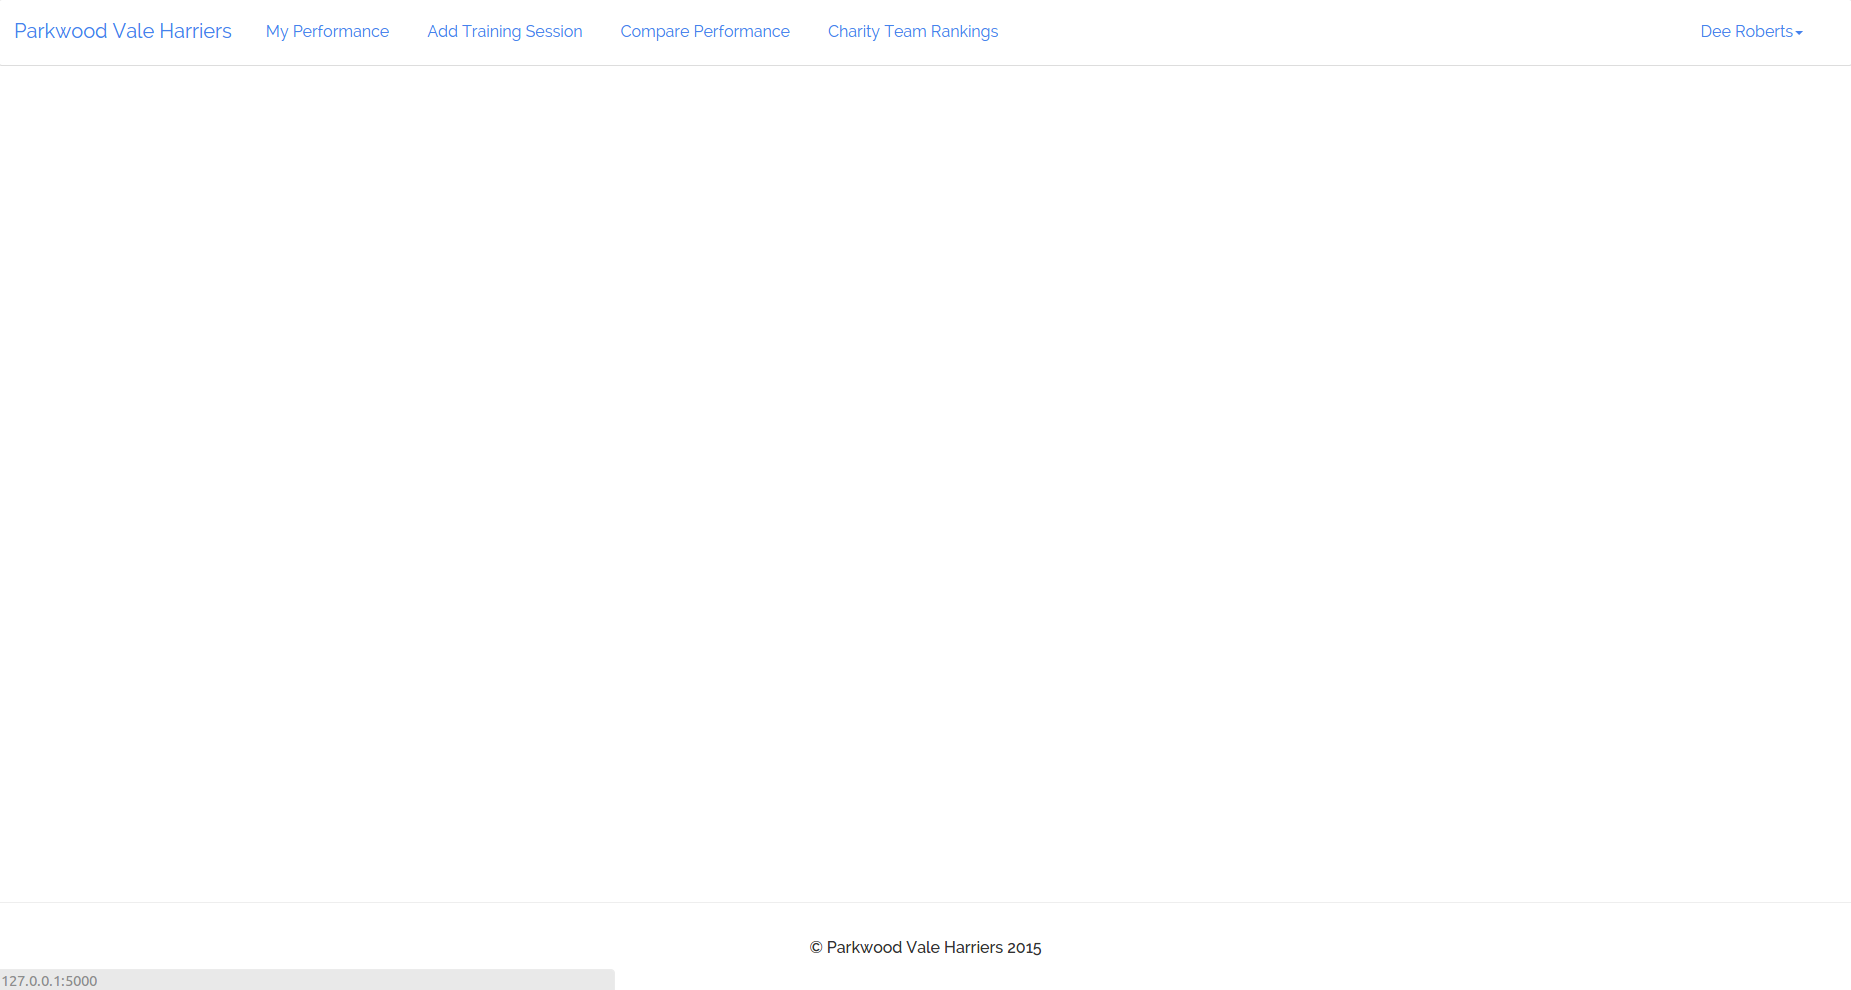
\includegraphics[scale=0.30]{final_ui/layout}
  \caption{Master Layout}
\end{figure}

\subsection{Register Page}
The register page features a clear, simple design, with input boxes laid out in a consistent style. Each input box features placeholder text, to provide a visual guide to the user as to what sort of data they should be typing in. To simplify entry, the date of birth input brings up a datepicker widget upon click, making it simple for users to enter their date of birth. Additionally, validation errors are featured at the top of the page in a big yellow box, making them easy to see; they also have a close button to prevent them getting in the way. A link to the login page allows users who already have an account to quickly login.

\begin{figure}[h!]
  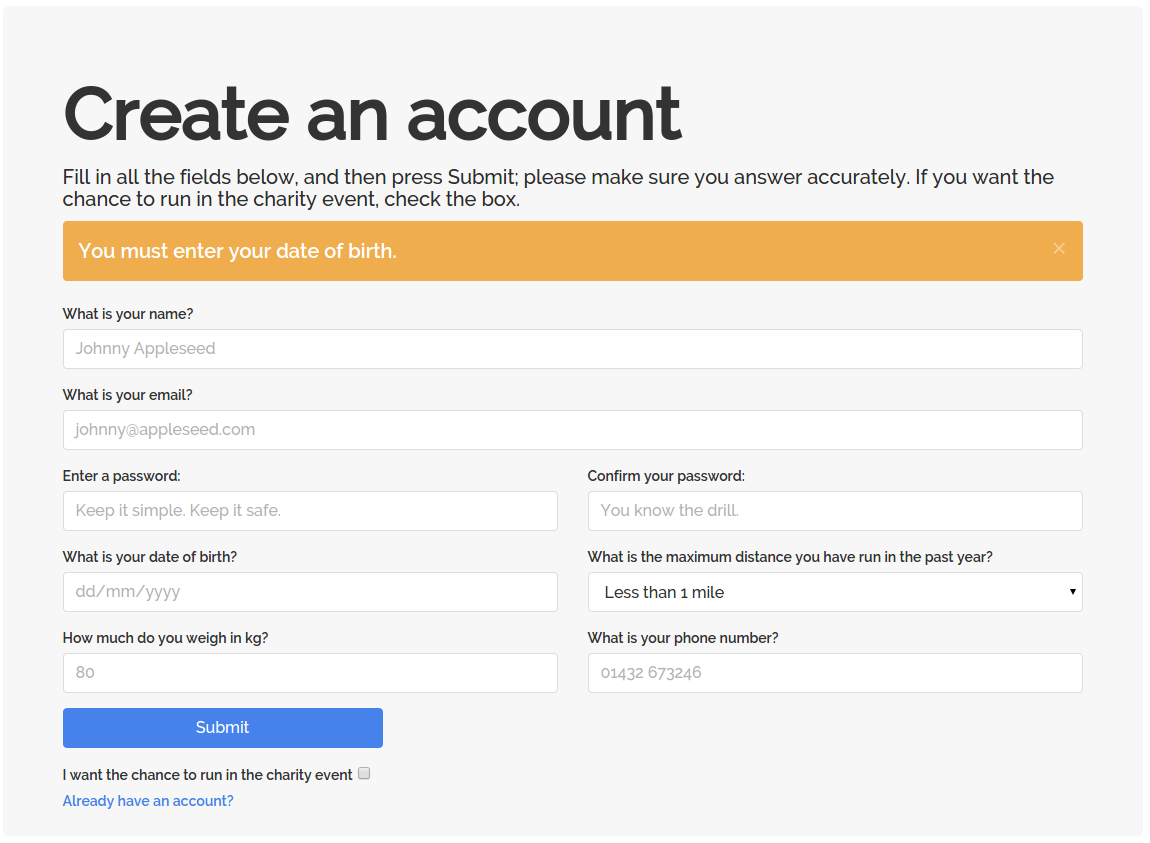
\includegraphics[scale=0.35]{final_ui/register}
  \caption{Registration Page}
\end{figure}
\clearpage

\subsection{Login Page}
As the login page has only one function - to get the user logged in to the system - it features a very simple layout, with only two input forms and a button. Like the registration form, though not visible in this capture, placeholders are overlaid on the inputs to provide a visual guide as to should be typed in. Additionally, the password field blanks out the input, a helpful security measure that prevents onlookers viewing the user's password. For consistency, the same validation error system as with the registration page is used.

\begin{figure}[h!]
  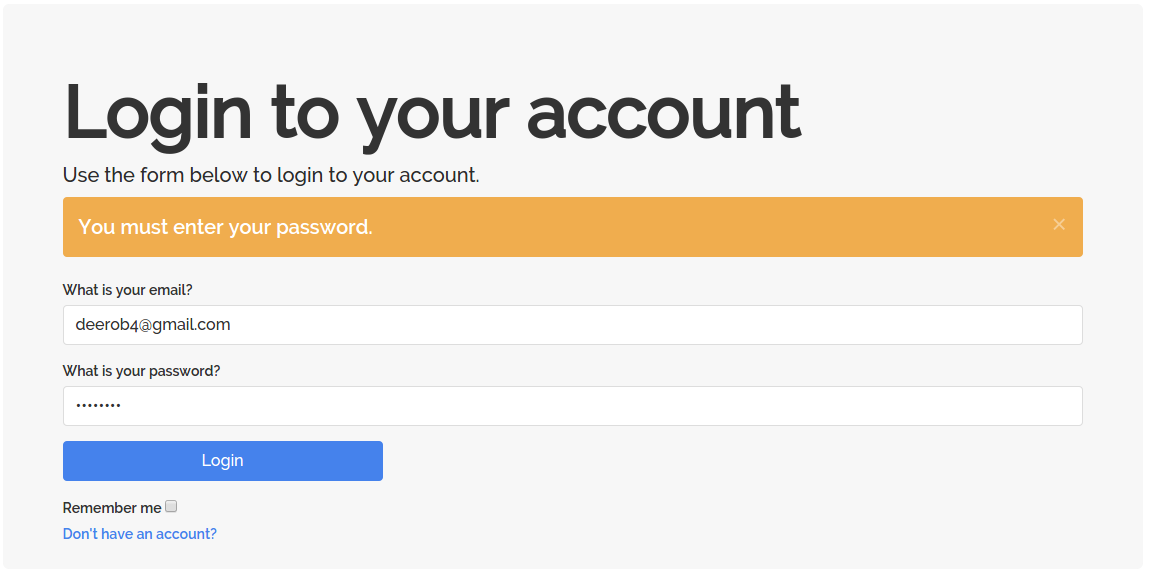
\includegraphics[scale=0.35]{final_ui/login}
  \caption{Login Page}
\end{figure}
\clearpage

\subsection{Profile Page}
The profile page allows the user to view and update their personal information. Certain sections appear on demand, so multiple captures have been taken.

\subsubsection{Main View}
Due to the large amount of data that is being presented on this page, a structured approach has been taken, with a three-panel view being implemented. This helps to seperate the different areas of the page in a logical manner, making it easier for the user to find what they are looking for. Each item of data is given its own row, making it clear which is which. The delete account section has been coloured in red, a colour traditionally associated with danger. This helps to convey to the user that bad things will happen if they delete their account. Furthermore, playful text has been used in the delete account panel, to bring a sense of amusement and, hopefully, dissuade the user from following through with their actions.

\begin{figure}[h!]
  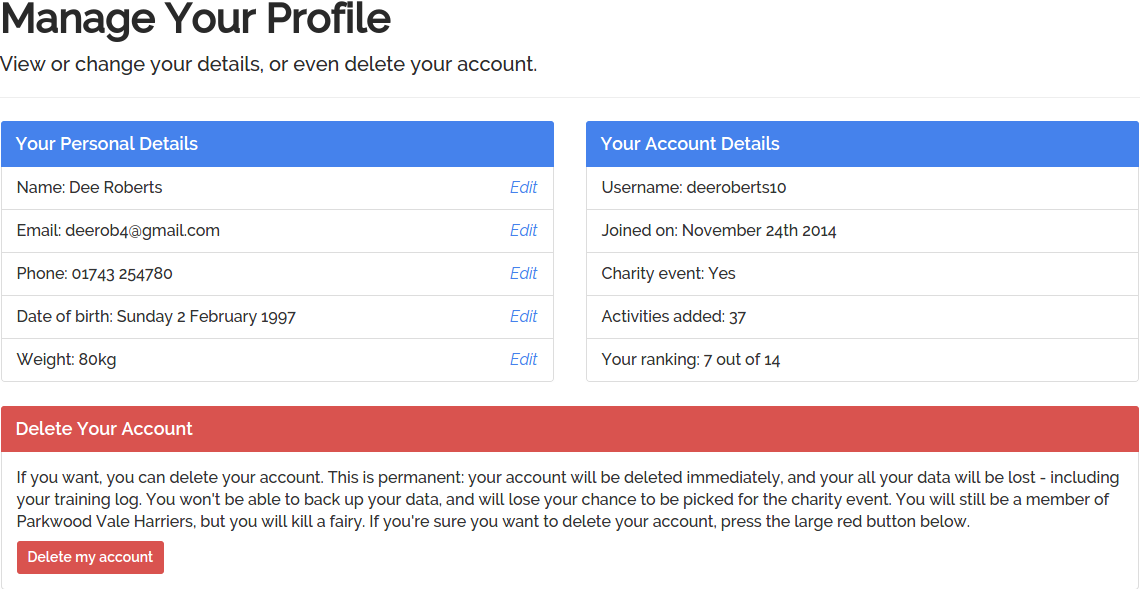
\includegraphics[scale=0.35]{final_ui/profile}
  \caption{Profile Page - Main View}
\end{figure}
\clearpage

\subsubsection{Change Details}
The interface for changing details is very simple - it features just an input for changing the element, and a button to confirm. The placeholder text for the input is set to the current item, for visual consistency. Making this panel pop up as opposed to being on a seperate page improves the flow of the page, preventing the user becoming disorientated.

\begin{figure}[h!]
  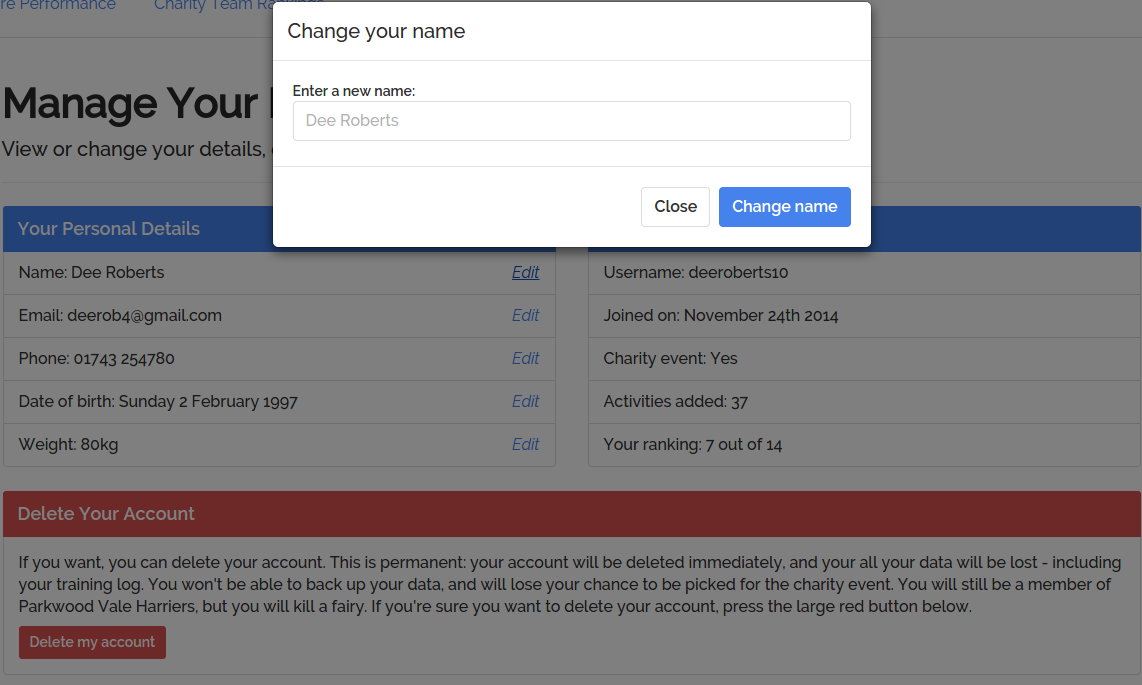
\includegraphics[scale=0.35]{final_ui/profile_change}
  \caption{Profile Page - Change Details}
\end{figure}
\clearpage

\subsubsection{Delete Account}
To ensure that the user is fully aware of the severity of deleting their account, they must type in "I will lose everything" into the box; this also makes it harder for them to accidentally delete their account. Positive reinforcement is used in this section through the use of colours - greeen is associated with positivity, and users have been shown to click on green coloured buttons more often than red; this further dissuades them from deleting their account.

\begin{figure}[h!]
  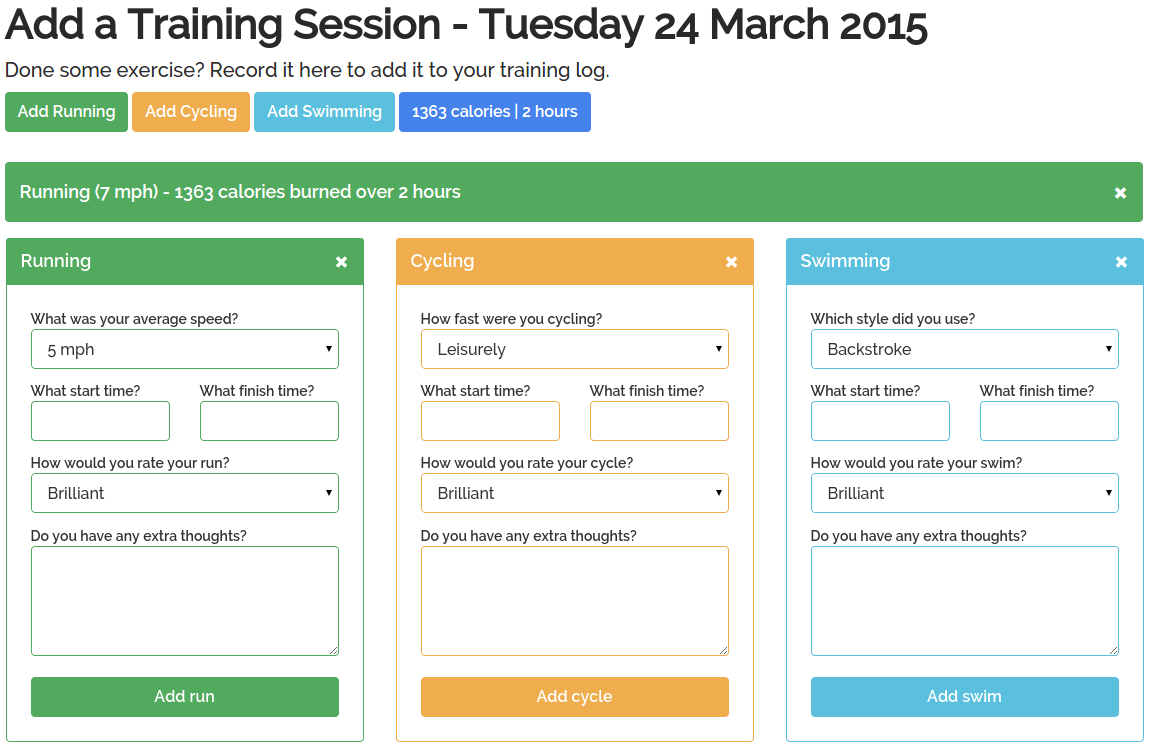
\includegraphics[scale=0.35]{final_ui/account_delete}
  \caption{Profile Page - Delete Account}
\end{figure}

\subsection{User Performance Page}
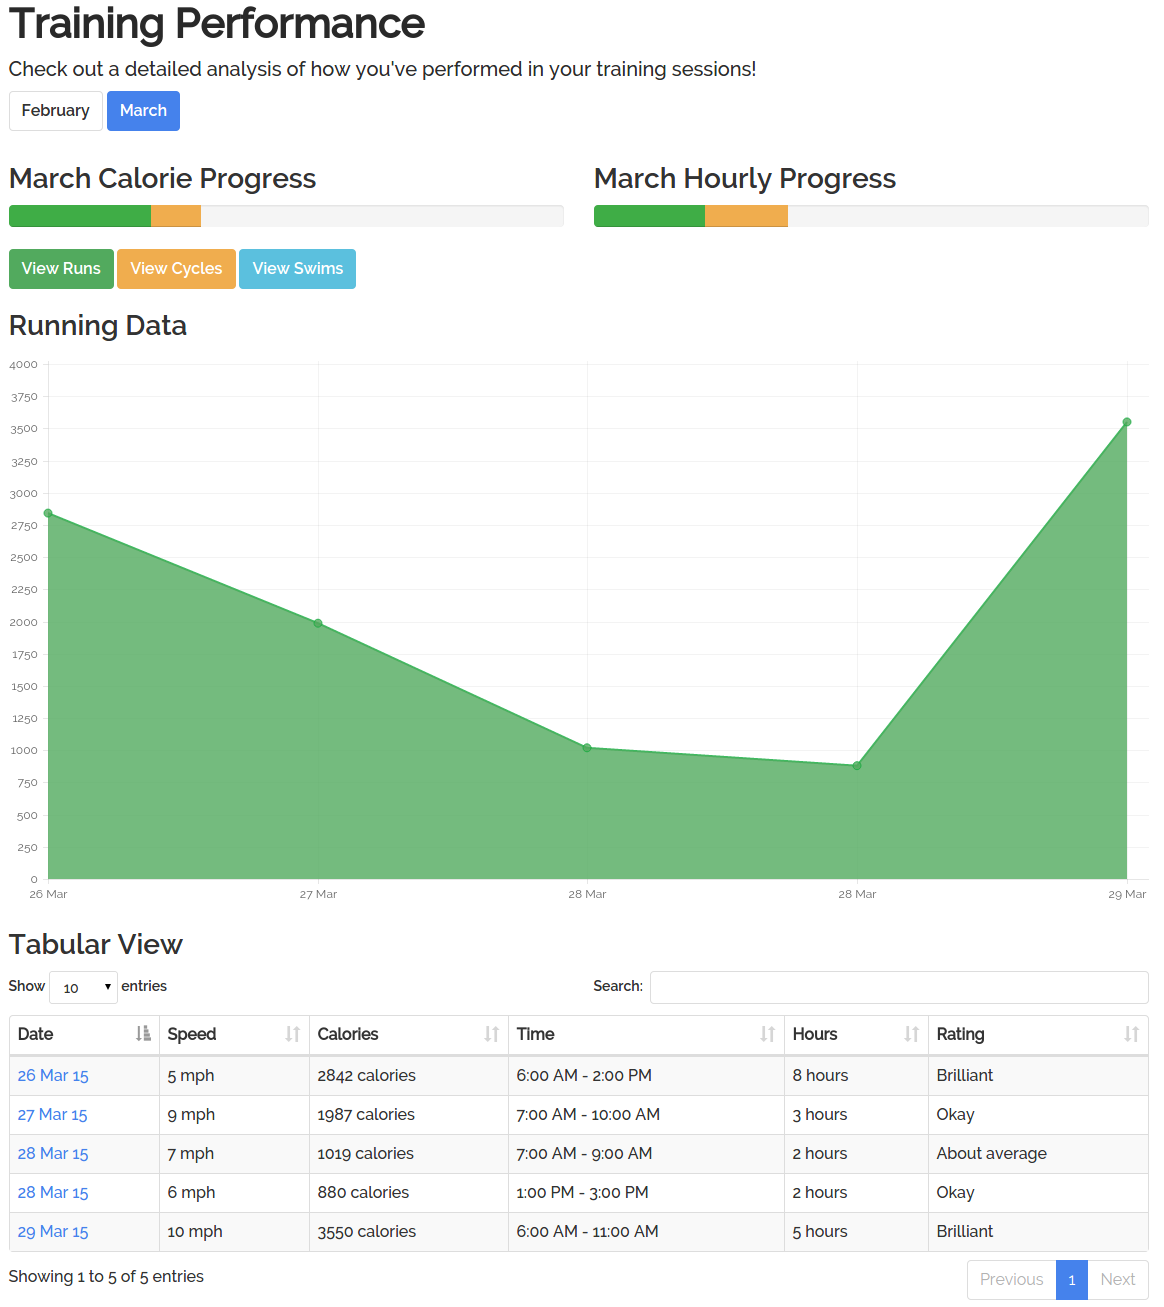
\includegraphics[scale=0.35]{final_ui/user_performance}

\subsection{Add Activity Page}
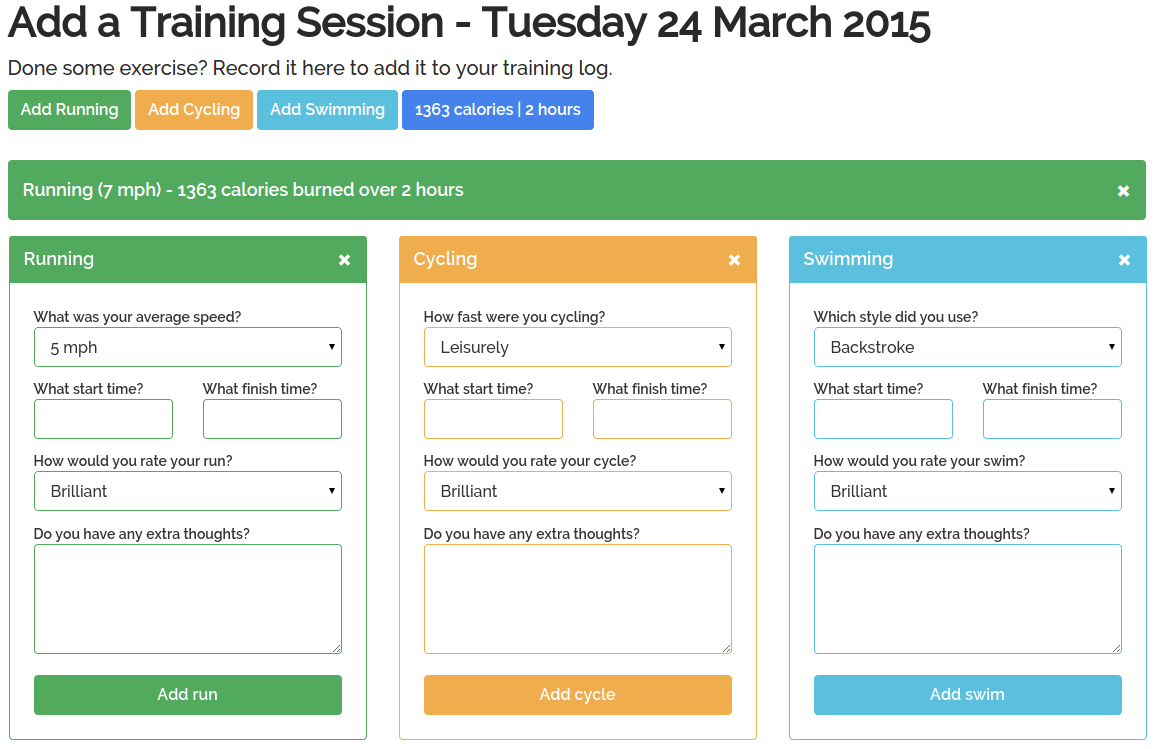
\includegraphics[scale=0.35]{final_ui/add_activity}

\subsection{Rankings Page}
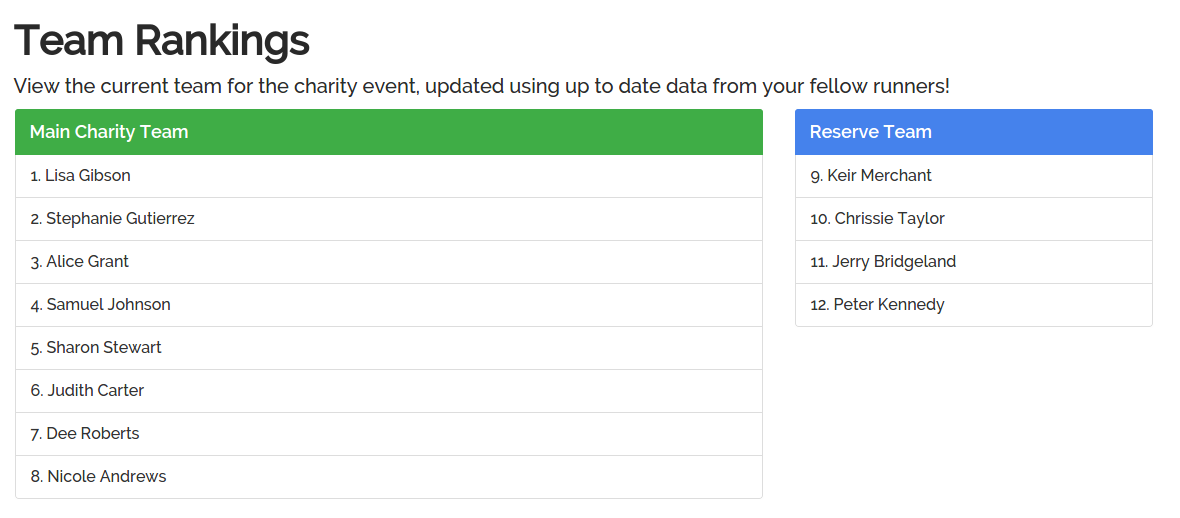
\includegraphics[scale=0.35]{final_ui/rankings}

\section{Database Models}
This section contains documentation on the finished database tables and models, including an ER diagram showing the relationship between the tables, schematics, and a visual view.

\subsection{Table Relationships}
The activities and users are linked through a foreign key This means that there is a one to many relationship between users and activities - one user can have many activities, but each activity can only have one user.

\begin{figure}[h!]
  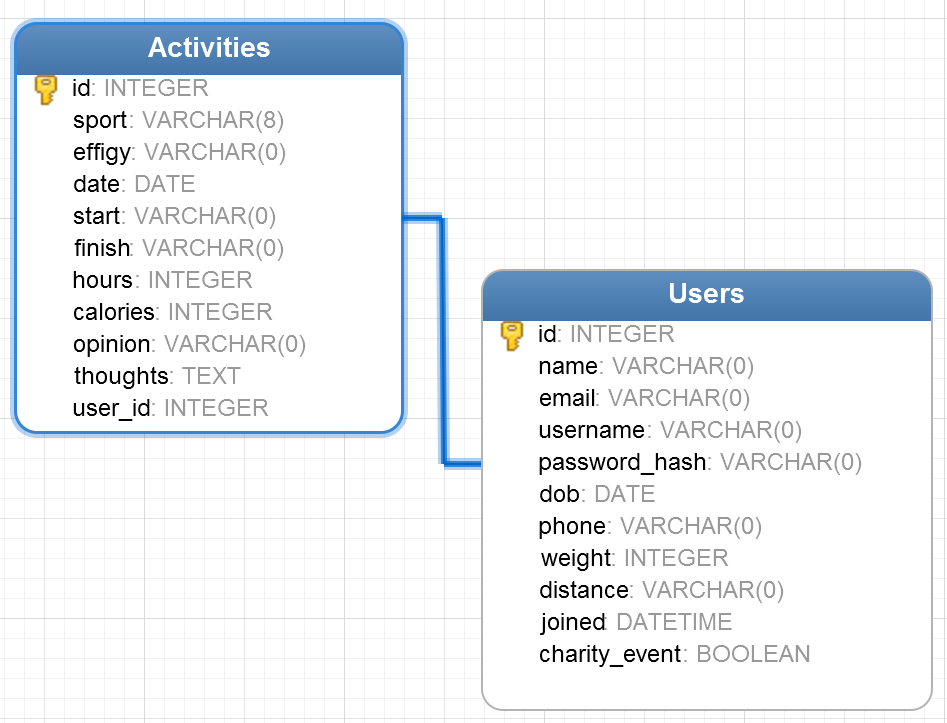
\includegraphics[scale=0.5]{images/database/er_diagram}
  \caption{Table Relationships}
\end{figure}

\clearpage

\subsection{Table Schemas}
Each table in the database has its own schema, in which is described the name, data type and key type of each column. They can be found below.

\subsubsection{Users Table}
The id column is the primary key. Email is used to login. Username is used in certain routes; see processes. Weight is used to calculate calories.
\begin{figure}[h!]
  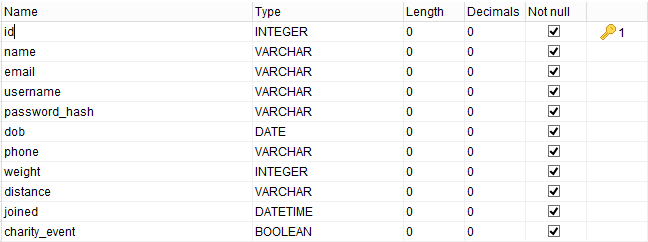
\includegraphics[scale=0.65]{images/database/users_schema}
  \caption{Users Table Schema}
\end{figure}

\subsubsection{Activities Table}
The id column is the primary key. Effigy is the specific details of each activity, such as the swimming stroke or running speed. user\_id is the foreign key linking the activity to a user.
\begin{figure}[h!]
  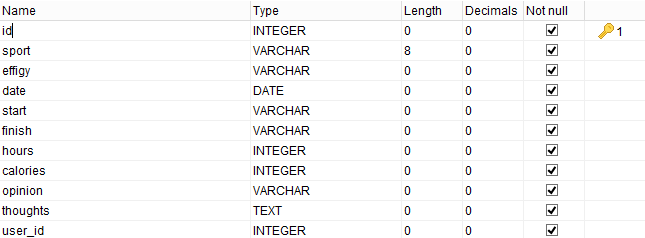
\includegraphics[scale=0.65]{images/database/activities_schema}
  \caption{Activities Table Schema}
\end{figure}

\clearpage

\subsection{Data Views}
The following is a snapshot of the data in the two tables at the time of writing, to illustrate how they will appear in production.

\subsubsection{Users Table}
\begin{figure}[h!]
  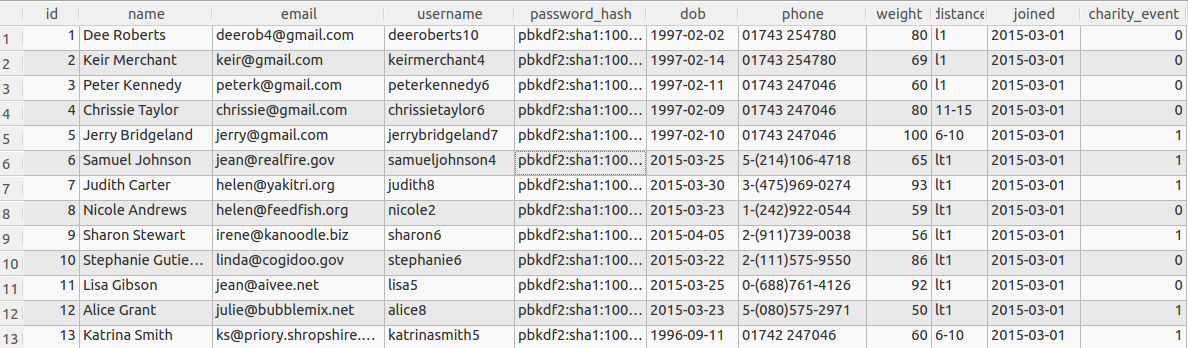
\includegraphics[scale=0.37]{images/database/users_visual}
  \caption{Users Table Data View}
\end{figure}

\subsubsection{Activities Table}
\begin{figure}[h!]
  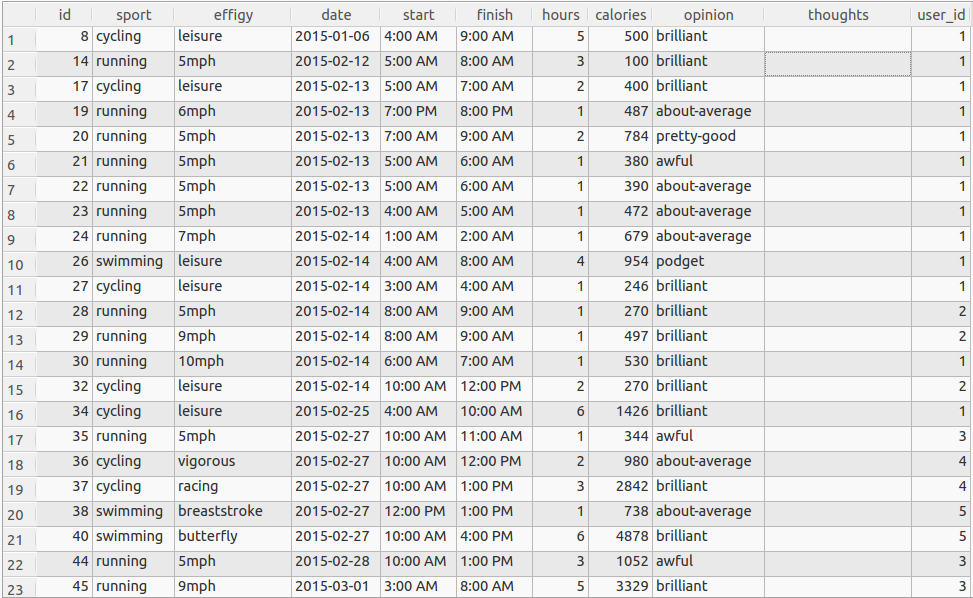
\includegraphics[scale=0.37]{images/database/activities_visual}
  \caption{Activities Table Data View}
\end{figure}

\section{Variables}
A very large number of variables have been used throughout the system in order to store data temporarily. It should be noted that variables in Python do not work in the same way as in other languages like Visual Basic: a variable acts as a pointer to something already in memory (created by Python automatically), as opposed to creating a space in memory to store the contents of the variable. Therefore, the code x = 10 merely sets the variable x to an address that points at 10, as opposed to writing 10 into memory.

\subsection{Global Variables}
Throughout the system, a small number of global variables are used in order to provide functionality. The following table lists their names, type and purpose.
\begin{table}[h]
\begin{tabular}{|l|l|l|}
\hline
\textbf{Name} & \textbf{Type} & \textbf{Purpose}                        \\ \hline
login\_manager                    & Object                 & Creates the actual Flask application object.     \\ \hline
db                     & Object                 & Returns a connection to the database.            \\ \hline
User                   & Object                 & Creates a connection to the Users db table.      \\ \hline
Activity               & Object                 & Creates a connection to the Activities db table. \\ \hline
current\_user          & Object                 & Returns details about the logged in user.        \\ \hline
\end{tabular}
\caption{Global Variables}
\end{table}

\subsection{Local Variables}
The following table contains a list of all the variables used locally throughout the functions / classes.
\begin{table}[h]
\begin{tabular}{lllll}
\textbf{Name}     & \textbf{Type} & \textbf{File Found} & \textbf{Function / Class} & \textbf{Purpose}                        \\
login\_manager    & Object        & \_init\_.py         & create\_app             & Creates the login object.               \\ \hline
name              & Object        & forms.py            & MemberForm              & Creates the name input.                 \\ \hline
dob               & Object        & forms.py            & MemberForm              & Creates the dob input.                  \\ \hline
password          & Object        & forms.py            & MemberForm              & Creates the password input.             \\ \hline
confirm           & Object        & forms.py            & MemberForm              & Creates the confirm input.              \\ \hline
charity\_event    & Object        & forms.py            & MemberForm              & Creates the charity input.              \\ \hline
distance          & Object        & forms.py            & MemberForm              & Creates the distance input.             \\ \hline
weight            & Object        & forms.py            & MemberForm              & Creates the weight input.               \\ \hline
phone             & Object        & forms.py            & MemberForm              & Creates the phone input,                \\ \hline
submit            & Object        & forms.py            & MemberForm              & Creates the submit button.              \\ \hline
age               & int           & forms.py            & validate\_dob           & Stores the user's age.                  \\ \hline
email             & Object        & forms.py            & LoginForm               & Creates the email input.                \\ \hline
password          & Object        & forms.py            & LoginForm               & Creates the password input.             \\ \hline
remember          & Bool          & forms.py            & LoginForm               & Creates the remember input.             \\ \hline
login             & Object        & forms.py            & LoginForm               & Creates the login button.               \\ \hline
id                & Object        & models.py           & User                    & Creates the id column.                  \\ \hline
name              & Object        & models.py           & User                    & Creates the name column.                \\ \hline
email             & Object        & models.py           & User                    & Creates the email column.               \\ \hline
username          & Object        & models.py           & User                    & Creates the username column.            \\ \hline
password\_hash    & Object        & models.py           & User                    & Creates the hash column.                \\ \hline
dob               & Object        & models.py           & User                    & Creates the dob column.                 \\ \hline
phone             & Object        & models.py           & User                    & Creates the phone column.               \\ \hline
weight            & Object        & models.py           & User                    & Creates the weight column.              \\ \hline
distance          & Object        & models.py           & User                    & Creates the distance column.            \\ \hline
joined            & Object        & models.py           & User                    & Creates the joined column.              \\ \hline
charity\_event    & Object        & models.py           & User                    & Creates the charity column.             \\ \hline
activities        & Object        & models.py           & User                    & Creates relationship property.          \\ \hline
id                & Object        & models.py           & Activity                & Creates the id column.                  \\ \hline
sport             & Object        & models.py           & Activity                & Creates the effigy column.              \\ \hline
date              & Object        & models.py           & Activity                & Creates the date column.                \\ \hline
start             & Object        & models.py           & Activity                & Creates the start column.               \\ \hline
finish            & Object        & models.py           & Activity                & Creates the finish column.              \\ \hline
hours             & Object        & models.py           & Activity                & Creates the hours column.               \\ \hline
calories          & Object        & models.py           & Activity                & Creates the calories column.            \\ \hline
opinion           & Object        & models.py           & Activity                & Creates the opinion column.             \\ \hline
thoughts          & Object        & models.py           & Activity                & Creates the thoughts column.            \\ \hline
user\_id          & Object        & models.py           & Activity                & Creates the user\_id column.            \\ \hline
today             & Date          & helpers.py          & calculate\_age          & Stores the current date.                \\ \hline
months            & List          & perf\_data.py       & perf\_data              & Stores a list of months.                \\ \hline
all\_activities   & Object        & per\_data.py        & perf\_data              & Stores all the user's sessions.         \\ \hline
all\_runs         & Object        & per\_data.py        & perf\_data              & Stores all the user's runs.             \\ \hline
all\_cycles       & Object        & per\_data.py        & perf\_data              & Stores all the user's cycles.           \\ \hline
all\_swims        & Object        & per\_data.py        & perf\_data              & Stores all the user's swims.            \\ \hline
month\_map        & Dict          & per\_data.py        & perf\_data              & Maps months to integers.                \\ \hline
calorie\_goal     & int           & per\_data.py        & perf\_data              & Stores the calorie goal.                \\ \hline
hour\_goal        & int           & per\_data.py        & perf\_data              & Stores the hourly goal.                 \\ \hline
sport             & String        & ajax.py             & sport\_block            & Stores the type of sport                \\ \hline
sport             & String        & ajax.py             & send\_activity          & Retrieves the sport                     \\ \hline
effiy             & String        & ajax.py             & send\_activity          & Retrieves the effigy                    \\ \hline
hours             & int           & ajax.py             & send\_activity          & Retrieves the hours                     \\ \hline
start             & int           & ajax.py             & send\_activity          & Retrieves the start                     \\ \hline
finish            & int           & ajax.py             & send\_activity          & Retrieves the finish                    \\ \hline
opinion           & String        & ajax.py             & send\_activity          & Retrieves the opinion                   \\ \hline
thoughts          & String        & ajax.py             & send\_activity          & Retrieves the thoughts                  \\ \hline
activity          & Object        & ajax.py             & send\_activity          & Stores the completed activity           \\ \hline
activity\_id      & int           & ajax.py             & remove\_activity        & Stores the id of the activity           \\ \hline
base\_calories    & Dict          & ajax.py             & calculate\_calories     & Stores the base calorie values          \\ \hline
sport             & String        & ajax.py             & calculate\_calories     & Retrieves the sport                     \\ \hline
effiy             & String        & ajax.py             & calculate\_calories     & Retrieves the effigy                    \\ \hline
hours             & int           & ajax.py             & calculate\_calories     & Retrieves the hours                     \\ \hline
start             & int           & ajax.py             & calculate\_calories     & Retrieves the start                     \\ \hline
finish            & int           & ajax.py             & calculate\_calories     & Retrieves the finish                    \\ \hline
opinion           & String        & ajax.py             & calculate\_calories     & Retrieves the opinion                   \\ \hline
thoughts          & String        & ajax.py             & calculate\_calories     & Retrieves the thoughts                  \\ \hline
base\_value       & int           & ajax.py             & calculate\_calories     & Stores the base value for activity      \\ \hline
calories          & int           & ajax.py             & calculate\_calories     & Stores the total calories               \\ \hline
modifier          & int           & ajax.py             & calculate\_calories     & Stores the correct calorie modifier     \\ \hline
activity\_data    & Dict          & ajax.py             & calculate\_calories     & Stores all the activity data            \\ \hline
month\_map        & Dict          & ajax.py             & user\_charts            & Stores a mapping of months to int       \\ \hline
runs              & Object        & ajax.py             & user\_charts            & Stores all the user's runs              \\ \hline
cycles            & Object        & ajax.py             & user\_charts            & Stores all the user's cycles            \\ \hline
swims             & Object        & ajax.py             & user\_charts            & Stores all the user's swims             \\ \hline
activity\_data    & Dict          & ajax.py             & user\_charts            & Stores calories and dates for charts    \\ \hline
month             & String        & ajax.py             & user\_charts            & Stores the requested month              \\ \hline
user\_data        & Dict          & ajax.py             & user\_charts            & Stores the performance data of user.    \\ \hline
form              & Object        & auth.py             & register                & Stores instance of class MemberForm     \\ \hline
username          & String        & auth.py             & register                & Stores the inputted username.           \\ \hline
user              & Object        & auth.py             & register                & Stores a User object with data          \\ \hline
form              & Object        & auth.py             & login                   & Stores instance of class LoginForm      \\ \hline
user              & Object        & auth.py             & login                   & Stores details of user with email       \\ \hline
only\_letters     & String        & main.py             & profiles                & Stores regexp to check valid name       \\ \hline
valid\_email      & String        & main.py             & profiles                & Stores regexp to check valid email      \\ \hline
valid\_phone      & String        & main.py             & profiles                & Stores regexp to check valid phone      \\ \hline
check\_integer    & String        & main.py             & profiles                & Stores regexp to check valid weight     \\ \hline
activity\_number  & int           & main.py             & profiles                & Stores number of activities of user     \\ \hline
total\_users      & int           & main.py             & profiles                & Stores the total number of users        \\ \hline
activities        & Object        & main.py             & add\_training           & Stores all activities for user on today \\ \hline
total\_calories   & int           & main.py             & add\_training           & Stores the total calories done today    \\ \hline
total\_hours      & int           & main.py             & add\_training           & Stores the total hours done today       \\ \hline
months            & List          & main.py             & performance             & Stores a list of months                 \\ \hline
all\_activities   & Object        & main.py             & performance             & Stores all activities for user          \\ \hline
available\_months & List          & main.py             & performance             & Stores months user has sessions in      \\ \hline
users             & Object        & main.py             & compare\_perf           & Stores all users who are charitable     \\ \hline
user\_list        & List          & main.py             & compare\_perf           & Stores sorted list of above users       \\ \hline
user\_ranking     & Dict / List   & main.py             & rankings                & Stores the best running team            \\ \hline
sport             & String        & ajax.py             & sport\_block              & Stores the type of sport                \\
sport             & String        & ajax.py             & send\_activity            & Retrieves the sport                     \\
effiy             & String        & ajax.py             & send\_activity            & Retrieves the effigy                    \\
hours             & int           & ajax.py             & send\_activity            & Retrieves the hours                     \\
start             & int           & ajax.py             & send\_activity            & Retrieves the start                     \\
finish            & int           & ajax.py             & send\_activity            & Retrieves the finish                    \\
opinion           & String        & ajax.py             & send\_activity            & Retrieves the opinion                   \\
thoughts          & String        & ajax.py             & send\_activity            & Retrieves the thoughts                  \\
activity          & Object        & ajax.py             & send\_activity            & Stores the completed activity           \\
activity\_id      & int           & ajax.py             & remove\_activity          & Stores the id of the activity           \\
base\_calories    & Dict          & ajax.py             & calculate\_calories       & Stores the base calorie values          \\
sport             & String        & ajax.py             & calculate\_calories       & Retrieves the sport                     \\
effiy             & String        & ajax.py             & calculate\_calories       & Retrieves the effigy                    \\
hours             & int           & ajax.py             & calculate\_calories       & Retrieves the hours                     \\
start             & int           & ajax.py             & calculate\_calories       & Retrieves the start                     \\
finish            & int           & ajax.py             & calculate\_calories       & Retrieves the finish                    \\
opinion           & String        & ajax.py             & calculate\_calories       & Retrieves the opinion                   \\
thoughts          & String        & ajax.py             & calculate\_calories       & Retrieves the thoughts                  \\
base\_value       & int           & ajax.py             & calculate\_calories       & Stores the base value for activity      \\
calories          & int           & ajax.py             & calculate\_calories       & Stores the total calories               \\
modifier          & int           & ajax.py             & calculate\_calories       & Stores the correct calorie modifier     \\
activity\_data    & Dict          & ajax.py             & calculate\_calories       & Stores all the activity data            \\
sport             & String        & ajax.py             & sport\_block              & Stores the type of sport                \\
sport             & String        & ajax.py             & send\_activity            & Retrieves the sport                     \\
effiy             & String        & ajax.py             & send\_activity            & Retrieves the effigy                    \\
hours             & int           & ajax.py             & send\_activity            & Retrieves the hours                     \\
start             & int           & ajax.py             & send\_activity            & Retrieves the start                     \\
finish            & int           & ajax.py             & send\_activity            & Retrieves the finish                    \\
opinion           & String        & ajax.py             & send\_activity            & Retrieves the opinion                   \\
thoughts          & String        & ajax.py             & send\_activity            & Retrieves the thoughts                  \\
activity          & Object        & ajax.py             & send\_activity            & Stores the completed activity           \\
activity\_id      & int           & ajax.py             & remove\_activity          & Stores the id of the activity           \\
base\_calories    & Dict          & ajax.py             & calculate\_calories       & Stores the base calorie values          \\
sport             & String        & ajax.py             & calculate\_calories       & Retrieves the sport                     \\
effiy             & String        & ajax.py             & calculate\_calories       & Retrieves the effigy                    \\
hours             & int           & ajax.py             & calculate\_calories       & Retrieves the hours                     \\
start             & int           & ajax.py             & calculate\_calories       & Retrieves the start                     \\
finish            & int           & ajax.py             & calculate\_calories       & Retrieves the finish                    \\
opinion           & String        & ajax.py             & calculate\_calories       & Retrieves the opinion                   \\
thoughts          & String        & ajax.py             & calculate\_calories       & Retrieves the thoughts                  \\
base\_value       & int           & ajax.py             & calculate\_calories       & Stores the base value for activity      \\
calories          & int           & ajax.py             & calculate\_calories       & Stores the total calories               \\
modifier          & int           & ajax.py             & calculate\_calories       & Stores the correct calorie modifier     \\
activity\_data    & Dict          & ajax.py             & calculate\_calories       & Stores all the activity data            \\
month\_map        & Dict          & ajax.py             & user\_charts              & Stores a mapping of months to int       \\
runs              & Object        & ajax.py             & user\_charts              & Stores all the user's runs              \\
cycles            & Object        & ajax.py             & user\_charts              & Stores all the user's cycles            \\
swims             & Object        & ajax.py             & user\_charts              & Stores all the user's swims             \\
activity\_data    & Dict          & ajax.py             & user\_charts              & Stores calories and dates for charts    \\
month             & String        & ajax.py             & user\_charts              & Stores the requested month              \\
user\_data        & Dict          & ajax.py             & user\_charts              & Stores the performance data of user.    \\
form              & Object        & auth.py             & register                  & Stores instance of class MemberForm     \\
username          & String        & auth.py             & register                  & Stores the inputted username.           \\
user              & Object        & auth.py             & register                  & Stores a User object with data          \\
form              & Object        & auth.py             & login                     & Stores instance of class LoginForm      \\
user              & Object        & auth.py             & login                     & Stores details of user with email       \\
only\_letters     & String        & main.py             & profiles                  & Stores regexp to check valid name       \\
valid\_email      & String        & main.py             & profiles                  & Stores regexp to check valid email      \\
valid\_phone      & String        & main.py             & profiles                  & Stores regexp to check valid phone      \\
check\_integer    & String        & main.py             & profiles                  & Stores regexp to check valid weight     \\
activity\_number  & int           & main.py             & profiles                  & Stores number of activities of user     \\
total\_users      & int           & main.py             & profiles                  & Stores the total number of users        \\
activities        & Object        & main.py             & add\_training             & Stores all activities for user on today \\
total\_calories   & int           & main.py             & add\_training             & Stores the total calories done today    \\
total\_hours      & int           & main.py             & add\_training             & Stores the total hours done today       \\
months            & List          & main.py             & performance               & Stores a list of months                 \\
all\_activities   & Object        & main.py             & performance               & Stores all activities for user          \\
available\_months & List          & main.py             & performance               & Stores months user has sessions in      \\
users             & Object        & main.py             & compare\_perf             & Stores all users who are charitable     \\
user\_list        & List          & main.py             & compare\_perf             & Stores sorted list of above users       \\
user\_ranking     & Dict / List   & main.py             & rankings                  & Stores the best running team            \\
sport             & String        & main.js             & \$sport-click             & Stores requested sport type             \\
\$start           & Object        & main.js             & validateActivity          & Stores the start time input             \\
\$finish          & Object        & main.js             & validateActivity          & Stores the finish time input            \\
\$activity        & Object        & main.js             & updateActivities          & Stores the activity panel               \\
sport             & String        & main.js             & animateActivity           & Stores the session sport                \\
containerWidth    & int           & main.js             & animateActivity           & Stores the width of the screen          \\
start             & Date          & main.js             & calculateHours            & Stores the inputted start time          \\
finish            & Date          & main.js             & calculateHours            & Stores the inputted finish time         \\
effigy            & String        & main.js             & calculateCalories         & Stores the effigy of training session   \\
rating            & String        & main.js             & calculateCalories         & Stores the rating of training session   \\
start             & String        & main.js             & calculateCalories         & Stores the start time of session        \\
finish            & String        & main.js             & calculateCalories         & Stores the finish time of session       \\
thoughts          & String        & main.js             & calculateCalories         & Stores the thoughts of training session \\
hours             & String        & main.js             & calculateCalories         & Stores the hours of training session    \\
caloriesBurned    & int           & main.js             & addActivity               & Stores the calories burned by session   \\
currentCalories   & int           & main.js             & addActivity               & Stores the day's current calories       \\
currentHours      & int           & main.js             & addActivity               & Stores the day's current hours          \\
activityString    & String        & main.js             & addActivity               & Stores the string to display in session \\
runningCtx        & Object        & ind\_charts.js      & constructChart            & Stores the running graph canvas         \\
swimmingCtx       & Object        & ind\_charts.js      & constructChart            & Stores the swimming graph canvas        \\
cyclingCtx        & Object        & ind\_charts.js      & constructChart            & Stores the cycling graph canvas         \\
runningData       & Object        & ind\_charts.js      & constructChart            & Stores the data for the running graph   \\
cyclingData       & Object        & ind\_charts.js      & constructChart            & Stores the data for the cycling graph   \\
swimmingData      & Object        & ind\_charts.js      & constructChart            & Stores the data for the swimming graph  \\
runningChart      & Object        & ind\_charts.js      & constructChart            & Stores the running chart                \\
cyclingChart      & Object        & ind\_charts.js      & constructChart            & Stores the cycling chart                \\
swimmingChart     & Object        & ind\_charts.js      & constructChart            & Stores the swimming chart              
\end{tabular}
\end{table}

\section{Annotated Listings}
This section contains all of the code for the system, split into several logical categories. The system is made up of a very large number of Python functions, as well as some additional aspects, such as Jinja2 HTML templates to display the interface, and CSS to provide styling.

\subsection{HTML Views}
Every page of the system has its own corresponding HTML template. These are used to display the data passed by the Python back-end, and provide interface elements such as buttons and dropdown boxes. A comparison can be drawn between them and the XML built by the Design Mode in Visual Basic, but, as thesealso contain some logic of their own, such as for-loops to loop through arrays, it is appropriate to include them in the documentation.

\subsubsection{layout.html}
\lstinputlisting[language=HTML, caption=Main Layout]{../app/templates/layout.html}

\subsubsection{register.html}
\lstinputlisting[language=HTML, caption=Register Page]{../app/templates/auth/register.html}

\subsubsection{login.html}
\lstinputlisting[language=HTML, caption=Login Page]{../app/templates/auth/login.html}

\subsubsection{user\_performance.html}
\lstinputlisting[language=HTML, caption=User Performance Page]{../app/templates/performance/user_performance.html}

\subsubsection{own\_profile.html}
\lstinputlisting[language=HTML, caption=User Profile Page]{../app/templates/profiles/own_profile.html}

\subsubsection{add\_training.html}
\lstinputlisting[language=HTML, caption=Add Training Session Page]{../app/templates/training/add_training.html}

\subsubsection{compare\_performance.html}
\lstinputlisting[language=HTML, caption=Compare Performance]{../app/templates/performance/compare_performance.html}

\subsubsection{rankings.html}
\lstinputlisting[language=HTML, caption=Rankings Page]{../app/templates/training/rankings.html}

\subsubsection{running\_block.html}
\lstinputlisting[language=HTML, caption=Running Block]{../app/templates/training/running_block.html}

\subsubsection{cycling\_block.html}
\lstinputlisting[language=HTML, caption=Cycling Block]{../app/templates/training/cycling_block.html}

\subsubsection{swimming\_block.html}
\lstinputlisting[language=HTML, caption=Swimming Block]{../app/templates/training/swimming_block.html}


\subsection{JavaScript Functions}
The system makes use of some JavaScript in order to create links between the front-end (the HTML files above) and the Python functions. Very little processing is done here; mainly data is transmitted back and forth between the client and the server.

\subsubsection{main.js}
\lstinputlisting[language=JavaScript, caption=Main JavaScript Functions]{../app/static/js/main.js}

\subsubsection{individual\_charts.js}
\lstinputlisting[language=JavaScript, caption=User Charts]{../app/static/js/individual_charts.js}


\subsection{CSS Styling}
A master CSS file is used to provide styling for the system, setting out things like the typography, layout and a little animation in places.

\lstinputlisting[caption=main.css]{../app/static/css/main.css}

\subsection{Python Processes}
The vast majority of the system is written in Python. These function handle everything from connecting and writing to the database, to calculating the number of calories burned in a training session, and everything in between. For a full rundown of what each function does, view the processes section.

\subsubsection{\_\_init\_\_.py}
This file handles very low level functions of the system, like creating and initialising the actual Flask application.
\lstinputlisting[language=Python, caption=\_\_init\_\_.py]{../app/__init__.py}

\subsubsection{forms.py}
This file defines the input forms used in the login and register pages. It sets the validation for each input, and defines the appropriate HTML element.
\lstinputlisting[language=Python, caption=forms.py]{../app/forms.py}

\subsubsection{models.py}
This file defines the database models used by the database. It sets up aspects like foreign/primary keys, and the data type of each column.
\lstinputlisting[language=Python, caption=models.py]{../app/models.py}

\subsubsection{helpers.py}
This file defines several smaller helper functions used multiple times throughout the system.
\lstinputlisting[language=Python, caption=helpers.py]{../app/helpers.py}

\subsubsection{performance\_data.py}
This file returns a JSON object containing all the training sessions for a user in a particular month. It is used throughout the system to return training data for use in tables and graphs.
\lstinputlisting[language=Python, caption=performance\_data.py]{../app/performance_data.py}

\subsubsection{auth.py}
This file defines the routes and processes used in the login / register process. They were placed in their own file for efficiency, and because they play a different part to others.
\lstinputlisting[language=Python, caption=auth.py]{../app/controllers/auth.py}

\subsubsection{ajax.py}
This file defines the routes used by the AJAX calls in the JavaScript files. All of these return a value, usually a JSON object, that is then used to dynamically update the page.
\lstinputlisting[language=Python, caption=ajax.py]{../app/controllers/ajax.py}

\subsubsection{main.py}
This file defines the majority of routes used by the system.
\lstinputlisting[language=Python, caption=main.py]{../app/controllers/main.py}

\cleardoublepage


\part{Testing and Evaluation}

\addcontentsline{toc}{section}{Unnumbered Section}

\end{document}